\chapter{Practical Concepts} \label{ch:concepts}
This chapter presents practical concepts, which were introduced in order to solve the refinement issues in \jecdar. Not all of the considered concepts have proven to be correct or suitable, such as concepts of arrival zone, min/max, accumulative delays and timeline. We show the problems these concepts were meant to solve and flaws of each of them. Finally we present the concept of a global zone which is the one currently used in \jecdar.

\section{Zone unions} \label{sec:zoneUnions}

The data structure that we use for representing clock constraints, the DBM, is very powerful and efficient for our purposes. Until now, the operations that we needed to perform on zones(e.g., apply constraint, delay, intersection) did not cause any issues.

A problem arose when we discovered the need to add multiple zones together in order to see "the full zone" for which a certain action is enabled. DBMs "have a well-known shortcoming: they are not closed under set-union. This comes from the fact that a set represented by a DBM is convex, while the union of two convex sets is not necessarily convex", as explained in \textcite{UppaalSecrets}.

This means that if we must perform addition or subtraction on DBMs, we must find a different data structure to store the result. The most logical approach, if we are to keep using DBMs, is to introduce the concept of zone union. On top of this, the DBM library provides support for zone unions, which simplifies the task for us.

\textcite{UppaalSecrets} also mentions that with a different data structure for zones, namely CDDs (Clock Difference Diagrams), performing operations such as addition or subtraction of zones would not be a problem, as these are closed under set-union. In spite of this, as long is there is no library support for CDDs, it is more convenient for us to continue using DBMs.

\section{Absolute zone}
The very first big concept that has been introduced in the project is \textit{absolute zone}. The concept was summoned to solve a number of problems related to the verification of the availability of an edge in the context of one or more automata trying to move simultaneously to a new state in case of refinement and other features. Further we list issues that were meant to be solved by an absolute zone:
\begin{itemize}
    \item Edge availability in an individual automaton given two or more clocks that are constrained such that an edge cannot be taken.
    \item Edge availability given that the constrained clocks (at least two) might end up having greatly differing possible valuations at some point of the state space exploration. 
    \item Transition (number of edges) availability in the case of two or more automata performing a simultaneous move in such features as Refinement, Composition and Conjunction.
    \item Adjustment of resulting arrival zones given that two or more automata move simultaneously, resulting in arrival zones having to be constrained according to the rules of Refinement, Composition and Conjunction.
\end{itemize}

Generally, an absolute zone should be used during the call to the \textsc{GetNextTransitions()} method described in \textcite{Jecdar:2019}, which returns transitions with all the possible moves from one state to another for an arbitrary amount of automata. It is also important to state that unlike arrival, invariant or guard zone, an absolute zone is not meant to be stored, but rather helps to properly manage the rest of the zones when taking an edge.

\subsection{Examples}
To be able to understand some of the issues better, consider the automaton in Figure \ref{fig:az-first}. Due to the fact that \textbf{id0} is an initial location, the arrival zones state that both of the clocks \textbf{x} and \textbf{y} begin from the value \textbf{0}. In such a scenario an output edge leading to location \textbf{id1} cannot be taken because of the non-intersecting guards for clocks with identical arrival zones. However, constraining the invariant zone with the guards would result in a completely valid zone (shown to the right of the automaton), tricking one into believing that the edge can be traversed.

\begin{figure}
\centering
\begin{tikzpicture}[thick,scale=0.9, every node/.style={scale=0.9}, baseline=0.5cm]
    \node[anchor=south west,inner sep=0] (image) at (0,0)
    {\includegraphics{figures/az-first.png}};
    \begin{scope}[x={(image.south east)},y={(image.north west)}]
        \node[font=\Large] at (-0.05,1.2) {$\bm{x[0;0 ]}$};
        \node[font=\Large] at (-0.05,0.8) {$\bm{y[0;0 ]}$};
        \node[font=\Large] at (0,-0.15) {$\bm{x[0;\infty )}$};
        \node[font=\Large] at (0,-0.55) {$\bm{y[0;\infty )}$};
        \node[font=\Large] at (0.45,-0.2) {$\bm{x[5;\infty )}$};
        \node[font=\Large] at (0.45,-0.6) {$\bm{y[0;4 )}$};
    \end{scope}
\end{tikzpicture} \hspace{1cm}
\begin{tabular}{c|c|c}
        $\leq 0$ & $\leq -5$ & $\leq 0$ \\
        \hline
        $\leq \infty$ & $\leq 0$ & $\leq \infty$ \\
        \hline
        $< 4$ & $< -1$ & $\leq 0$\\
   \end{tabular}
\caption{Unavailable edge in a single automaton and a corresponding valid guard zone} \label{fig:az-first}
\end{figure}

Next, consider a more complex refinement example of two automata excerpts in Figure \ref{fig:az-ref}, where the automaton on the left is challenged to refine the one on the right starting from locations \textbf{id0} and \textbf{id2}. The arrival zones of the two mentioned locations appear to differ to such a significant extent where it might seem from the first glance that the refinement output rule would not hold. 

\begin{figure}
\centering
\begin{tikzpicture}[thick,scale=0.9, every node/.style={scale=0.9}]
    \node[anchor=south west,inner sep=0] (image) at (0,0)
    {\includegraphics{figures/az-second.png}};
    \begin{scope}[x={(image.south east)},y={(image.north west)}]
        \node[font=\Large] at (-0.05,0.8) {$\bm{x[0;0 ]}$};
        \node[font=\Large] at (0,-0.15) {$\bm{x[0;\infty )}$};
        \node[font=\Large] at (0.5,-0.2) {$\bm{x[5;\infty )}$};
        \node[font=\Large] at (0.68,0.9) {$\bm{x[5;\infty )}$};
        
        \node at (2,0.45) {\includegraphics{figures/az-third.png}};
        \node[font=\Large] at (1.45,0.8) {$\bm{x[400;400]}$};
        \node[font=\Large] at (1.5,-0.15) {$\bm{x[400;\infty )}$};
        \node[font=\Large] at (2,-0.2) {$\bm{x[402;\infty )}$};
        \node[font=\Large] at (2.2,1.1) {$\bm{x[405;\infty )}$};
    \end{scope}
\end{tikzpicture}
\caption{Abstract example of an available transition where left automaton refines right automaton} \label{fig:az-ref}
\end{figure}

However, we will discover that the refinement output rule holds in this example. It is explained as follows; the automaton on the left must wait at least \textbf{5} time units before being able to issue an output, whereas the automaton on the right can always follow due to it being able to issue an output after delaying for at least two time units. Additionally, the arrival zone of the second automaton in \textbf{id3} must be adjusted to reflect that an edge was traversed only after delaying for at least \textbf{5} time units, since the right side of the refinement only follows the left side.

\begin{figure}
\centering
\begin{tabular}{c|c}
        $\leq 0$ & $\leq -5$  \\
        \hline
        $\leq \infty$ & $\leq 0$ \\
\end{tabular}
\hspace{2cm}
\begin{tabular}{c|c}
        $\leq 0$ & $\leq -2$  \\
        \hline
        $\leq \infty$ & $\leq 0$ \\
\end{tabular}
\caption{Absolute zones for automata from Figure \ref{fig:az-ref}} \label{fig:az-ref-zones}
\end{figure}

Figure \ref{fig:az-ref-zones} demonstrates two absolute zones that were built for the automata from the example in Figure \ref{fig:az-ref}. The key difference between the absolute zone and such zones as arrival, invariant or guard one, is its independence from the potentially fluctuating values of the arrival zone. The absolute zone is read as follows: the lower bound of a clock states the minimum amount of delay that is necessary to take before the edge becomes available. At least two time units must pass in order to be able to take an edge from location \textbf{id2} to \textbf{id3}, exactly which is reflected in the lower bound of the corresponding absolute zone. 

Oppositely, the upper bound of the clock in the absolute zone states the maximum possible delay that can be done while the edge still remains available. 


\subsection{Implementation details}
Now that we have seen some examples of the issues that the absolute zone is hoped to solve, we will take a look at the algorithm used to compute absolute zones. The function in Algorithm \ref{alg:absolute-zone} demonstrates the main logic used to calculate absolute zones given an invariant zone and the guards of an edge that is challenged for availability.

\begin{algorithm}
\caption{Algorithm to compute absolute zones}
\label{alg:absolute-zone}
\begin{algorithmic}[1]
\Function{getAbsoluteZone}{$invZone, guards$}
\State $absZone \gets invariantZone$
\ForAll{$guard$ in $guards$}
\State $constraint \gets \textsc{BoundToRaw}(guard.value)$
\State $clockLB \gets invZone.clockLB$
\State $clockUB \gets invZone.clockUB$
\If{(firstVisit)}
\State $absZone.\textsc{FreeDown}(guard.clock)$
\EndIf
	\If{($guard \in \{<,\leq \}$)}
        \If{($constraint > clockUB \And clockUB \neq \infty$)}
	        \State $NewUB \gets \textsc{addRawRaw}(clockUB, clockLB)$
	    \Else
	        \State $NewUB \gets \textsc{addRawRaw}(constraint, clockLB)$
	    \EndIf
	    \State $absZone.\textsc{ContstrainDBM(NewUB)}$
	\EndIf
		
	\If{($guard \in \{>,\geq \}$)}
	    \If{($constraint - clockLB < 0$)}
	        \State $NewLB \gets 0$
	    \Else
	        \State $NewLB \gets \textsc{addRawRaw}(constraint, clockLB)$
	    \EndIf
	     \State $absZone.\textsc{ContstrainDBM(NewLB)}$
	\EndIf
\EndFor
\ForAll{$clock$ in $unmodifiedClocks$}
\State $clockLB \gets invZone.clockLB$
\State $clockUB \gets invZone.clockUB$
\If{($clockLB \neq 1$)}
    \State $absZone.\textsc{FreeDown}(clock)$
\EndIf
\If{($clockUB \neq \infty$)}
\State $newUB \gets \textsc{addRawRaw}(clockUB, clockLB)$
\EndIf
\State $absZone.\textsc{ContstrainDBM(NewUB)}$
\EndFor
\State
\State \textbf{return $absZone$}	
\EndFunction
\end{algorithmic}
\end{algorithm}

Overall, the intent is to consider and treat respectively three cases of guards: guards that define the upper bound of the clock (Line 9), guards that define the lower bound of the clock (Line 15) and the absence of guards for certain clocks as such (Line 21). The first two cases related to different guards are treated in the first \textit{for all} loop (Lines 3-20), which is then followed by necessary changes to the bounds of the clocks that had no guards associated with them (Lines 21-28).

First of all, we assign three variables that are essential for further computations - \textit{constraint, clockUB} and \textit{clockLB} (Lines 4-6). Note that these variables are all of type \textbf{raw\_t} and correspond to the DBM library encoded constraints explained in Section \ref{sec:raw-values}. The \textsc{BoundToRaw()} method is used to encode the bounds of the guard into the required encoded constraint.

Due to the fact that constraining any bound of the clock will change the zone only if the applied constraint would tighten the zone, it is necessary to reset the lower bound of the clock that the guard is associated with, but only when that specific clock is handled for the first time (Lines 7-8).

Furthermore, depending on the type of the inequality symbol of the guard, the corresponding bound (upper bound or lower bound) must be calculated and then used to constrain the clock (Lines 10-14 and 16-20). Similarly, for clocks that were not constrained by any of the guards, a lower bound of the resulting zone's clock is freed, whereas its upper bound becomes the difference between the upper and lower bounds of the clock. 

The reason the difference is computed with the help of the \textsc{AddRawRaw()} DBM method is the handy fact that the lower bound constraints result in being encoded as negative raw values. Therefore, the addition of positive $clockUB$ and negative $clockLB$ in Lines 13, 19 and 27 will yield the correct result.

\subsection{Application of absolute zone}
The information contained in the generated absolute zone helps to solve the issues described above. Regardless of the values of the arrival zone and other zones derived from it, we now possess "absolute" information about the time intervals when an edge can be traversed. 

In the case of refinement it becomes a trivial task to check if one side of the refinement is able to follow the other one. To do so, one must compute the highest minimum delay value and the smallest maximum delay value among all clocks. The two resulting \textit{min} and \textit{max} values will represent the minimum delay and the maximum delay that can be taken among all clocks. After the computation is done for both sides of the refinement, it suffices to check the following two conditions:
\begin{itemize}
    \item $min_l \geq min_r$\\
    Check if an edge becomes available on the right side of the refinement earlier or at the same time as on the left side
    \item $max_l \leq max_r$\\
    Check if an edge remains available on the right side for at least as long as on the left side
\end{itemize}

\subsection{Absolute zone issues}
As we will discover later on, the concept of the absolute zone appears to have certain flaws and blind spots.

First of all, historically, the concept of absolute zones appeared and was implemented before the strictness fix, described in Section \ref{sec:strictnessFix}. This means that any addition or subtraction of constraints was a primitive operation due to constant "weak" strictness. From math we know that the addition and subtraction of weak constraints always results in a weak constraint. Due to this fact, the algorithm of the absolute zone did not encounter any issues in its frequently occurring addition or subtraction operations on raw values.

However, together with the strictness fix new problems arose. One of the issues expected to be solved, namely the adjustment of the resulting arrival zones, became impossible to perform correctly without losing or adding solutions to the zones, neither of which are acceptable in terms of correctness. 

\medskip

Moreover, absolute zones do not infer any information from arrival zones and therefore a lot of vital information is lost in the process. Consider the example in Figure \ref{fig:az-identical} where the upper automaton is challenged to refine the bottom one. It is also shown that both invariant and guard zones are absolutely identical in both cases. This means that the algorithm would produce identical absolute zones and naturally, after comparing the resulting \textit{min} and \textit{max} values, we deduce that the refinement holds. 

However, that is not the case in this example! It is easy to show that the refinement cannot hold due to the violation of the refinement output rule, which is caused by the only difference between the two automata - the reset on the edge from \textbf{id0} to \textbf{id1}. Consider having delayed \textbf{250} at location \textbf{id0} and outputting afterwards, resulting at \textit{id1}. The second automaton then follows according to the refinement output rule and gets to \textbf{id4}. Due to the above-mentioned reset, the upper automaton is able to delay up to \textbf{500} time units and output, whereas the bottom one, having arrived with the clock value of \textbf{250} already, will not be able to comply to the left side of the refinement.

Therefore, the concept of the absolute zone alone is not enough to handle all rules of refinement correctly.

\begin{figure}
\centering
\begin{tikzpicture}[thick,scale=0.9, every node/.style={scale=0.9}]
    \node[anchor=south west,inner sep=0] (image) at (0,0)
    {\includegraphics{figures/az-identical.png}};
    \begin{scope}[x={(image.south east)},y={(image.north west)}]
        
        \node[font=\Large] at (0.4,1) {$\bm{x[0;0]}$};
        \node[font=\Large] at (0.48,0.6) {$\bm{x[0;\infty )}$};
        \node[font=\Large] at (0.7,0.6) {$\bm{x[0;500]}$};
        
        \node[font=\Large] at (0.38,0.34) {$\bm{x[0;250]}$};
        \node[font=\Large] at (0.48,-0.05) {$\bm{x[0;\infty )}$};
        \node[font=\Large] at (0.7,-0.05) {$\bm{x[0;500]}$};
    \end{scope}
\end{tikzpicture}
\caption{The refinement of two almost identical automata that does not hold. Upper automaton refines bottom one.} \label{fig:az-identical}
\end{figure}

\section{Concept of Min/Max and zone union subtraction}
After realizing the failure of absolute zones to solve all the issues in the refinement relation, a new idea arose, namely Min/Max. This concept would take into consideration the very minimum of the arrival zone as well as its maximum and compare them to the corresponding guard interval. This comparison is vital when we have a reset on one of the automata, since it shows if both of the automata can delay the same amount before taking a corresponding edge.

Equation \ref{eq:lrMinMax} shows the algorithm which calculates the final min and max values for the left and the right side. In this algorithm $lf$ stands for the left side final values and $rf$ for the right side final values, while $g$ and $a$ stands for guard and arrival zone respectively. After receiving the final min and max values for both of the sides, one has to perform a comparison between them in order to see if both of the sides can traverse an edge at any given value within their intervals. This comparison can be seen in Equation \ref{eq:comparison}.
\begin{multline}
\label{eq:lrMinMax}
\\
lfMin = gMin - aMax\\
lfMax = gMax - aMin\\
rfMin = gMin - aMin\\
rfMax = gMax - aMax\\
\end{multline}
\begin{multline}
\label{eq:comparison}
\\
lfMin \geq rfMin\\
lfMax \leq rfMax\\
\end{multline}
\subsection{Examples of Min/Max}
In order to better understand how the Min/Max algorithm works, it is helpful to look at a few examples. The previously mentioned refinement relation from Figure \ref{fig:az-identical} using absolute zones fails, so this case has to be solved using the Min/Max algorithm mentioned in Equation \ref{eq:lrMinMax}. We are interested in locations, right before the reset happens, namely \textbf{id1} and \textbf{id4}. After the calculations of the final values, which are shown in \ref{eq:calcK3K4}, one can see that one of the rules is not satisfied, thus the refinement does not hold.
\begin{multline}
\label{eq:calcK3K4}
\\
lfMin = 0 - 0 = 0\\
lfMax = 500 - 0 = 500\\
rfMin = 0 - 0 = 0\\
rfMax = 250 - 0 = 250\\
0 \geq 0 \\
500 \rlap{\kern.45em$|$}\leq 250 \\
\end{multline}

To ensure that the algorithm works correctly, one has to take a look at an example which is opposite to the previous one. Figure \ref{fig:K1K2} shows a refinement relation between two automata, the upper one refining the lower one. Imagine a scenario where one would delay at location \textbf{id0} until $x=500$ and then traverse the edge. The arrival value of \textbf{id1} would be $500$, while in location \textbf{id4} - $0$, due to the reset. This would break the refinement relation, since the upper automaton would be able to traverse the output edge \textbf{o!}, while the right side of refinement would not be able to follow, since it has to delay at least $250$ in order to traverse the corresponding edge.

\begin{figure}
\centering
\begin{tikzpicture}[thick,scale=0.9, every node/.style={scale=0.9}]
    \node[anchor=south west,inner sep=0] (image) at (0,0)
    {\includegraphics{figures/K1K2.png}};
    \begin{scope}[x={(image.south east)},y={(image.north west)}]
        
        \node[font=\Large] at (0.37,1) {$\bm{x[250;\infty)}$};
        \node[font=\Large] at (0.48,0.6) {$\bm{x[0;\infty )}$};
        \node[font=\Large] at (0.7,0.6) {$\bm{x[500;\infty)}$};
        
        \node[font=\Large] at (0.4,0.38) {$\bm{x[0;0]}$};
        \node[font=\Large] at (0.48,0.02) {$\bm{x[0;\infty )}$};
        \node[font=\Large] at (0.7,0) {$\bm{x[250;\infty)}$};
    \end{scope}
\end{tikzpicture}
\caption{The refinement of two almost identical automata that does not hold. Upper automaton refines bottom one.} \label{fig:K1K2}
\end{figure}
Knowing that the refinement relation does not hold, one can check if the Min/Max algorithm would provide the same results. Once again we must look at the location that has a reset preceding it. The calculation of Min/Max from locations \textbf{id1} and \textbf{id4} can be seen in Figure \ref{eq:calcK1K2}. The rule, which requires $lfMin \geq rfMin$ does not hold, thus the Min/Max algorithm provides the same results.
\begin{multline}
\label{eq:calcK1K2}
\\
lfMin = 500 - \infty = 0\\
lfMax = \infty - 250 = \infty\\
rfMin = 250 - 0 = 250\\
rfMax = \infty - 0 = \infty\\
0 \rlap{\kern.45em$|$}\geq 250 \\
\infty \leq \infty \\
\end{multline}

\subsection{Issues of Min/Max}
This algorithm solves all the problems where there is only one outgoing edge from each of the locations. However, when we start taking into consideration examples such as in Figure \ref{fig:H1H2}, where the automaton has more than one outgoing edge, the algorithm starts providing incorrect results. The exact scenario is when the left automaton refines the right one. Both of the edges on the right side combined are capable of covering output \textbf{o!} at any given point where the left side would output, thus the refinement holds in this case. However, if one would try to place the values into the Min/Max formula, it would break. Consequently, we need a new approach for dealing with multiple outgoing edges.

\begin{figure}
\centering
\begin{tikzpicture}[thick,scale=0.9, every node/.style={scale=0.9}]
    \node[anchor=south west,inner sep=0] (image) at (0,0)
    {\includegraphics{figures/H1H2.png}};
    \begin{scope}[x={(image.south east)},y={(image.north west)}]
        
        \node[font=\Large] at (-0.02,0.93) {$\bm{x[0;0]}$};
        \node[font=\Large] at (0.03,0.56) {$\bm{x[0;\infty )}$};
        \node[font=\Large] at (0.2,0.56) {$\bm{x[40;\infty)}$};
        
        \node[font=\Large] at (0.57,0.93) {$\bm{x[0;0]}$};
        \node[font=\Large] at (0.78,0.55) {$\bm{x[40;50 )}$};
        \node[font=\Large] at (0.78,0.03) {$\bm{x[50;\infty)}$};
    \end{scope}
\end{tikzpicture}
\caption{Multiple outgoing edges from a single location} \label{fig:H1H2}
\end{figure}

Previously in Section \ref{sec:zoneUnions}, we have discovered the existence of DBM unions which are called Federations. When working with Federations, the subtraction method can be used in order to check if one of the Federations does not cover some part of the zone. Using this new approach one can easily deal with covering the zones of multiple edges. With this newly obtained knowledge, we have improved the Min/Max algorithm to use subtraction of federations and slightly modified some of the formulas, which can be seen in Equation \ref{eq:newMinMax}. The new Min/Max algorithm made it possible to verify if the refinement relation holds even in cases with multiple outgoing edges for the same action.

\begin{multline}
\label{eq:newMinMax}
\\
fminmin = gMin - aMin\\
fminmax = gMax - aMin\\
fmaxmin = gMin - aMax\\
fmaxmax = gMax - aMax\\
left[fminmin;fminmax] - right[fminmin;fminmax] = \emptyset\\
left[fmaxmin;fmaxmax] - right[fmaxmin;fmaxmax] = \emptyset\\
\end{multline}
This algorithm was supposed to work properly, but we found out that there is an issue. Math rules state that subtraction cannot be used with two inequalities of the same sign, meaning that operations such as $min - min$ bounds or $max - max$ bounds cannot be performed.

\section{Accumulative delays} \label{sec:accumDelays}
Another issue that we faced while trying to implement refinement is accumulative delays. Such concept arises when there exists a composition on one of the sides of the refinement relation. During composition, multiple automata will have internal moves, which could have different delays with resets. When a reset happens in an internal move, one must keep track of how long it was possible to delay before taking such action, thus one has to perform an addition of delays for every single internal action that has delays. In order to better understand the issue, one may take a look at Figure \ref{fig:accDelay}.

If one would directly check the availability in time of the common actions in the refinement, then one could say that the refinement holds, since the right side can take the $go!$ action until $x<=76$, while the left side requires the output edge to be available only until $x<=30$. However, the relation must be analyzed from the very start, where multiple resets happen before the refinement move, when a common action is taken. The first move that is taken is from \textbf{id3} to \textbf{id4} with an output action $i!$, where the value of maximum possible delay, which is $27$, has to be kept because clock $x$ is being reset here. On the other side of the composition, the possible time of traversing the edge between \textbf{id0} and \textbf{id1} shrinks down from $\infty$ to $x<=27$. The next composition move is being performed from \textbf{id1} to \textbf{id2} with an output edge $i1!$, where the maximum possible delay is until $x<=20$, it shrinks down the right side's possibility to move from \textbf{id4} to \textbf{id5} from $\infty$. Here we have to perform the accumulation of delays, since we have a reset again. The first max delay which happened was $27$, while the second one was $20$, so the total is $47$. Finally, one has to perform a refinement move with the common action \textbf{go!}, where the delays have to be added once more, until the next internal moves are going to happen. The right side can take the \textbf{go!} edge, as long as $x<=30+47=77$, while the right side cannot comply to the last $x$ value, so the refinement relation does not hold in this case.

\begin{figure}
\centering
\begin{tikzpicture}[thick,scale=0.9, every node/.style={scale=0.9}]
    \node[anchor=south west,inner sep=0] (image) at (0,0)
    {\includegraphics{figures/accum-delays.png}};
    \begin{scope}[x={(image.south east)},y={(image.north west)}]
        
        \node[font=\Large] at (0.70,0.2) {$\Scale[2]{{\leq}}$};
        \node[font=\Large] at (0.32,0.65) {$\Scale[2]{{\parallel}}$};
    \end{scope}
\end{tikzpicture}
\caption{Refinement, which requires accumulative delays} \label{fig:accDelay}
\end{figure}

\subsection{Implementation details}
After seeing the issue and the basic idea of how it can be solved with an example, one can take a look at the algorithm which computes the accumulation of delays. The function in Algorithm \ref{alg:accumDelay} demonstrates the main logic used to calculate the internal delays, given the source state and the target state.

The very first thing that is checked, in line 2, is if there was a reset, which is done by checking if the arrival min and max values are equal to zero. This check is important, because the accumulation of delays should happen only after reset, since time moves linearly and one can see the maximum delays within the guard zone. If the reset did not happen, we set the delay sum of the target state (DSum) to be equal to guard's maximum. In line 3, we check if guard maximum is infinity or if our current DSum is equal to infinity, then we set our target's DSum to be equal to infinity. The else statement in line 5 simply adds up the source DSum with guard's maximum and stores it in the target's DSum. This accumulation has to be performed on both sides of the refinement, since both sides can have internal moves.

\begin{algorithm}
\caption{Algorithm to compute accumulation of delays}
\label{alg:accumDelay}
\begin{algorithmic}[1]
\Function{accumulateDelays}{$sourceState, targetState$}
\If {$(aMin == 0 \And aMax == 0)$} 
    \If {$(source.DSum == INF \parallel gMax == INF)$}
        \State $target.DSum \gets INF;$
    \Else
        \State $target.DSum \gets source.DSum + gMax;$
    \EndIf
\Else 
    \State $target.DSum \gets gMax;$
\EndIf
        
\EndFunction
\end{algorithmic}
\end{algorithm}

At the end of the day, there were no significant issues while using accumulative delays. However after introducing a new concept, which is described in Section \ref{sec:globalZone}, there was no need for accumulative delays anymore. The reasoning behind this is that Global zone can handle it without any external help from such a function. 


\section{Timeline}
After facing such concepts as the absolute zone, Min/Max values and not being able to compare zones of the two sides of the refinement with the help of zone union subtraction, due to the possibly differing amount of clocks on each side, it was decided to introduce a \textit{flattening} abstraction.

The idea originated from previous discoveries: one is not able to compare zones of the left and right side of the refinement. The subtraction or intersection of the zones that is required to verify refinement rules did not appear possible to be performed, not only due to differing clock sizes of the refinement sides, but also because those clocks cannot be semantically compared (related to each other). 

As a result, it is necessary to compare the relationship of a set of an arbitrary amount of clocks with another such set. To achieve that, we introduce the concept of the \textit{timeline}, which in principle allows to flatten a multidimensional zone into a single dimension representing common results. Consider Figure \ref{fig:tl-1}, where a simplistic automaton has only one output edge, but three different clocks - \textit{x, y} and \textit{z}. Since location \textbf{id0} is the initial one and has no invariant assigned to it, the arrival and invariant zones of all three clocks evaluate to \textbf{0} and allow to indefinitely delay in that location respectively. The observation of the arrival zone of the location \textbf{id1} is of great interest: each of the clocks is constrained by the guards related to the rest of the clocks. This happens due to natural synchronous time progress that is identical for all of the clocks.

\begin{figure}
\centering
\begin{tikzpicture}[thick,scale=0.9, every node/.style={scale=0.9}]
    \node[anchor=south west,inner sep=0] (image) at (0,0)
    {\includegraphics{figures/timeline-1.png}};
    \begin{scope}[x={(image.south east)},y={(image.north west)}]
        \node[font=\Large] at (0,1.4) {$\bm{x[0;0 ]}$};
        \node[font=\Large] at (0,1.1) {$\bm{y[0;0 ]}$};
        \node[font=\Large] at (0,0.8) {$\bm{z[0;0 ]}$};
        
        \node[font=\Large] at (0.02,0) {$\bm{x[0;\infty )}$};
        \node[font=\Large] at (0.02,-0.3) {$\bm{y[0;\infty )}$};
        \node[font=\Large] at (0.02,-0.6) {$\bm{z[0;\infty )}$};
        
        \node[font=\Large] at (0.3,-0.3) {$\bm{x(8;\infty )}$};
        \node[font=\Large] at (0.5,-0.3) {$\bm{y[2;30 ]}$};
        \node[font=\Large] at (0.7,-0.3) {$\bm{z[0;15 ]}$};
        
        \node[font=\Large] at (0.8,1.4) {$\bm{x(8;15 ]}$};
        \node[font=\Large] at (0.8,1.1) {$\bm{y(8;15 ]}$};
        \node[font=\Large] at (0.8,0.8) {$\bm{z(8;15 ]}$};
    \end{scope}
\end{tikzpicture}
\caption{Three clocks resulting is identical arrival zones after taking an edge} \label{fig:tl-aut}
\end{figure}

This observation evolved into the concept of flattening an arbitrary amount of clocks into a single "global" clock that represents all the possible clock valuations fot which an edge can be traversed. Figure \ref{fig:tl-1} shows an example of the timeline for the automaton in Figure \ref{fig:tl-aut}. Since the timeline can always be represented by one clock, we choose to draw it as an interval, where the values of the interval are derived from "tightest" guards. The semantics of the presented timeline is as follows: in order to traverse an edge from \textbf{id0} to \textbf{id1}, more than \textit{8} time units must pass ($x>8$ being the tightest lower bound constraint) and the edge remains traversable until \textit{15} ($z \leq 15$ being the tightest upper bound constraint).

\begin{figure}
\centering
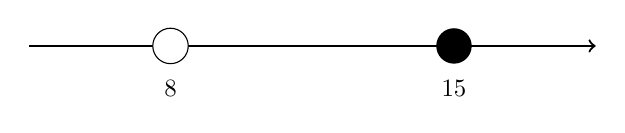
\begin{tikzpicture}[scale=0.9, every node/.style={scale=0.9}]
    \draw [thick ,->] (0,1) -- (8,1);
    \draw[fill=white] (2,1) circle (0.25);
    \node at (2,0.4) {$\bm{8}$};
    \fill (6,1) circle (0.25);
    \node at (6,0.4) {$\bm{15}$};
    \end{tikzpicture}

\caption{Timeline for the example in Figure \ref{fig:tl-aut}} \label{fig:tl-1}
\end{figure}

It is important to note that the concept of the timeline is also supposed to consider the fact that the refinement holds only when all the possible scenarios of state-space exploration satisfy its rules. The interval line(timeline) must reflect all the possible valuations that are common for all the clocks when the edge can be traversed, which includes all possible valuations for clocks derived from arrival zones.

\subsection{Implementation details}
To get a better intuition of what a timeline is and how it can be computed, consider the example in Figure \ref{fig:tl-plot}, where the arrival and guard zones are shown. As already mentioned, the arrival zone plays an important role in the computation of the resulting values of the timeline. 

\begin{figure}
\centering
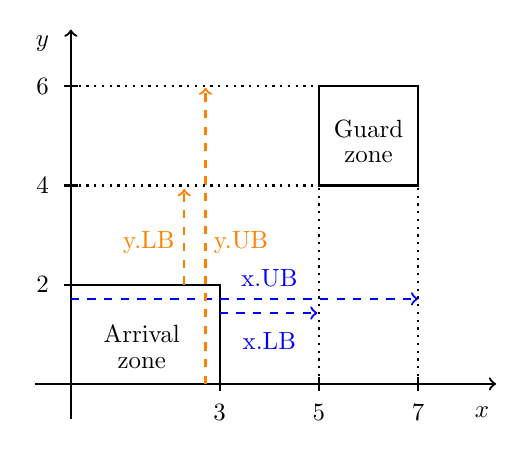
\begin{tikzpicture}[scale=0.9, every node/.style={scale=0.9}]
    % Axis
    \draw [thick ,->] (-0.5,0) -- (6,0);
    \draw [thick ,->] (0,-0.5) -- (0,5);
    \node at (5.8,-0.4) {$\bm{x}$};
    \node at (-0.4,4.8) {$\bm{y}$};
    
    % X coordinates
    \draw [thick] (2.1,-0.1) -- (2.1,0.1);
    \node at (2.1,-0.4) {$\bm{3}$};
    \draw [thick] (3.5,-0.1) -- (3.5,0.1);
    \node at (3.5,-0.4) {$\bm{5}$};
    \draw [thick] (4.9,-0.1) -- (4.9,0.1);
    \node at (4.9,-0.4) {$\bm{7}$};
    
    % Y coordinates
    \draw [thick] (-0.1,1.4) -- (0.1,1.4);
    \node at (-0.4,1.4) {$\bm{2}$};
    \draw [thick] (-0.1,2.8) -- (0.1,2.8);
    \node at (-0.4,2.8) {$\bm{4}$};
    \draw [thick] (-0.1,4.2) -- (0.1,4.2);
    \node at (-0.4,4.2) {$\bm{6}$};
    
    % Zones
    \draw [thick] (0,1.4) -- (2.1,1.4) -- (2.1, 0);
    \node at (1, 0.7) {Arrival};
    \node at (1, 0.3) {zone};
    \draw [thick] (3.5,2.8) -- (3.5,4.2) -- (4.9, 4.2) -- (4.9, 2.8) -- cycle;
    \node at (4.2, 3.6) {Guard};
    \node at (4.2, 3.2) {zone};
    
    % Dashed Arrows
    % Horizontal
    \draw [thick, blue, dashed, ->] (2.1,1) -- (3.48, 1);
    \draw [thick, blue, dashed, ->] (0,1.2) -- (4.9, 1.2);
    % Vertical
    \draw [thick, orange, dashed, ->] (1.9, 0) -- (1.9, 4.18);
    \draw [thick, orange, dashed, ->] (1.6,1.4) -- (1.6, 2.75);
    
    % Text on arrows
    \node[blue] at (2.8,0.6) {x.LB};
    \node[blue] at (2.8,1.5) {x.UB};
    
    \node[orange] at (1.1, 2) {y.LB};
    \node[orange] at (2.4, 2) {y.UB};
    
    % Dotted lines
    \draw [thick , dotted] (3.5,0) -- (3.5, 2.8);
    \draw [thick , dotted] (4.9,0) -- (4.9, 2.8);
    \draw [thick , dotted] (0,2.8) -- (3.5, 2.8);
    \draw [thick , dotted] (0,4.2) -- (3.5, 4.2);
    
\end{tikzpicture}
\caption{Computation of lower and upper bounds for further construction of a timeline.} \label{fig:tl-plot}
\end{figure}

Intuitively, the lower bound (LB) for a certain clock is the difference between the LB of the guard zone and the upper bound (UB) of the arrival zone for the respective clock. On the other hand, UB is the difference between the UB of the guard zone and the LB of the arrival zone for the respective clock.

Algorithm \ref{alg:timeline} demonstrates the computational process of the timeline. The idea is to compute the LBs and UBs for each of the clocks (Lines 4 and 5), and to pick the tightest bounds among all calculated LBs and UBs (Lines 10-13). The resulting two tightest bounds (final lower bound (FLB) and final upper bound (FUB) are the ones used to construct a timeline. Note that similarly to the previous algorithms, the difference between UB and LB is computed with the help of the addition function (\textsc{addRawRaw}), which is suitable due to the fact that the raw value of the LB is negative.

Also note that the resulting LB is expected to be a negative raw value, which is natural for all LBs. If the LB exceeds its allowed maximum value, it is set to the maximum value (Lines 6-7). This is a frequent example in cases where the arrival zone overlaps with the guard zone.

The UB also has its own minimum value, at most evaluating to \textbf{0} raw value. If the algorithm detects UB evaluating to negative raw values, it reports failure (Lines 8,9). This might happen in cases where the guard zone is "behind" the arrival zone in time, and therefore there are no clock valuations when an edge could be traversed.
\begin{algorithm}
\caption{Algorithm to compute timeline}
\label{alg:timeline}
\begin{algorithmic}[1]
\Function{getAbsoluteZone}{$arrZone, guardZone$}
\State $LB, UB, FLB = 1, FUB = Integer.MaxValue - 1;$
\ForAll{$clock$ in $zone$}
\State $LB \gets \textsc{addRawRaw}(arrZone.clockUB, guardZone.clockLB)$
\State $UB \gets \textsc{addRawRaw}(arrZone.clockLB, guardZone.clockUB)$
\If{($LB > 1$)}
\State $LB \gets 1$
\EndIf
\If{($UB < 1$)}
\State \textbf{return $null$}
\EndIf

\If{($LB < FLB$)}
\State $FLB \gets LB$
\EndIf
\If{($UB < FUB$)}
\State $FUB \gets UB$
\EndIf
\EndFor
\State
\State \textbf{return} new $Zone(1, FLB, FUB, 1)$
\EndFunction
\end{algorithmic}
\end{algorithm}

\subsection{Zone adjustment}
The timeline shows us absolute clock valuations during which an edge can be traversed and helps to verify if for all the solutions of one side of the refinement, the other side is able to "follow" by traversing an edge with the same action. However not only that, but the timeline can be used to adjust zones of both sides of the refinement.

Consider the automaton example in Figure \ref{fig:tl-autRight} which is the right side of the refinement, whereas the automaton of the left side of the refinement has been shown in Figure \ref{fig:tl-aut}. In order to construct a proper state pair of locations \textbf{id0} and \textbf{id3} for the refinement relation it is crucial to have proper zones to ensure the correctness of further state-space exploration, if any. 

The arrival zone at location \textbf{id3} in Figure \ref{fig:tl-autRight} which is depicted in red is an example of an incorrect zone in case of the refinement. Such zone would be correct if the automaton was explored outside the refinement relation or if it was on the left side of it. However, the timeline in Figure \ref{fig:tl-1} has shown that the output edge is traversed only in the interval of clock valuations from 8 (not included) until 15 (included). According to the refinement output rule, we are only interested in exploring such clock valuations on the right side as dictated by the left side. Therefore, the correct arrival zone would have to be $\bm{x(8;15]}$ (depicted in green).

\begin{figure}
\centering
\begin{tikzpicture}[thick,scale=0.9, every node/.style={scale=0.9}]
    \node[anchor=south west,inner sep=0] (image) at (0,0)
    {\includegraphics{figures/timeline-2.png}};
    \begin{scope}[x={(image.south east)},y={(image.north west)}]
        \node[font=\Large] at (-0.05,1) {$\bm{x[0;0 ]}$};
        \node[font=\Large] at (0.05,-0.2) {$\bm{x[0;\infty )}$};
        \node[font=\Large] at (0.5,0) {$\bm{x[0;\infty )}$};
        \node[font=\Large, green] at (0.7,1.25) {$\bm{x(8;15]}$};
        \node[font=\Large, red] at (0.7,0.85) {$\bm{x[0;\infty )}$};
        
    \end{scope}
\end{tikzpicture}
\caption{Automaton that is refined by the automaton from Figure \ref{fig:tl-aut}} \label{fig:tl-autRight}
\end{figure}

Such a  zone adjustment can be achieved by the following steps:
\begin{itemize}
    \item $LB_{AZ} = LB_{IZ} + LB_{timeline}$ \\
    To get the lower bound of the target arrival zone it is required to increase the source location invariant zone lower bound by the lower bound of the timeline.
    \item $UB_{AZ} = LB_{IZ} + UB_{timeline}$ \\
    Set the upper bound to be the same as the lower bound and then increase it by the upper bound of the timeline.
\end{itemize}

\subsection{Timeline issues}
In practice, the concept of timeline appeared to be capable of solving the same problems that absolute zones and min/max concepts did, but at a much more efficient and intuitive level. Unfortunately, it was discovered that the timeline has a number of flaws that prevent this concept from providing the expected results in some corner cases.

First of all, the information about the correct strictness may be lost after constructing a timeline. The example in Figure \ref{fig:tl-2} shows two cases where identical arrival zones and two different guard zones are used in each case to construct corresponding timelines. The resulting timelines appear to be identical, even though the strictness of the upper bound of the guards they were derived from differ. This is correct from the mathematical point of view, as the addition of two bounds, s.t. at least one of them is strict, will always result in a strict bound. However, in further computations that would result in incorrectly constructed arrival zones, as the information about exact strictness(one bound being non strict) is lost.


\begin{figure}
\centering
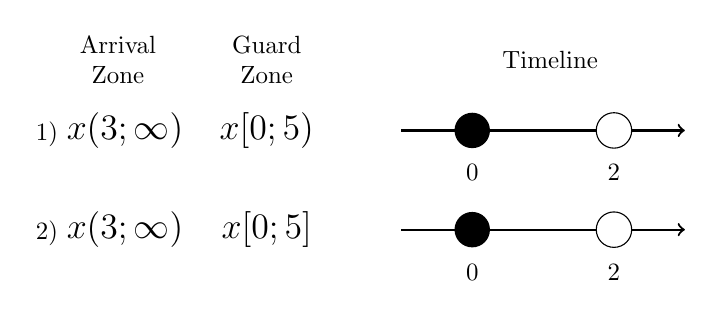
\begin{tikzpicture}[scale=0.9, every node/.style={scale=0.9}]

    \node[align=center] at (1,1) {Arrival \\ Zone};
    \node[align=center] at (3.1,1) {Guard \\ Zone};
    \node[align=center] at (7.1,1) {Timeline};
    \node at (0,-0.05) {1)};
    \node[font=\Large] at (1.1,0) {$\bm{x(3;\infty )}$};
    \node[font=\Large] at (3.1,0) {$\bm{x[0;5)}$};
    
    \node at (0,-1.45) {2)};
    \node[font=\Large] at (1.1,-1.4) {$\bm{x(3;\infty )}$};
    \node[font=\Large] at (3.1,-1.4) {$\bm{x[0;5]}$};
    
    
    \draw [thick ,->] (5,0) -- (9,0);
    \fill (6,0) circle (0.25);
    \draw[fill=white] (8,0) circle (0.25);
    \node at (6,-0.6) {$\bm{0}$};
    \node at (8,-0.6) {$\bm{2}$};
    
    \draw [thick ,->] (5,-1.4) -- (9,-1.4);
    \fill (6,-1.4) circle (0.25);
    \draw[fill=white] (8,-1.4) circle (0.25);
    \node at (6,-2) {$\bm{0}$};
    \node at (8,-2) {$\bm{2}$};
    \end{tikzpicture}

\caption{Two identical timelines for different strictness guards} \label{fig:tl-2}
\end{figure}

Secondly, we discovered that in some cases even if the timeline is correct, it does not anymore preserve the necessary information for the zone adjustment algorithm. Similarly to previous examples, Figure \ref{fig:tl-3} demonstrates four cases of arrival and guard zone combinations with varying strictness of the bounds. In fact, even though all the timelines are identical, they are absolutely correct according to their primary purpose. Each of them states that in all the possible scenarios of the state-space exploration joined together (which is driven by different arrival values), one might be able to traverse an edge immediately or to delay indefinitely and still be able to do so. However, such timeline is not suitable for proper zone adjustment as it has lost information about the necessary delay in some of the cases.

\begin{figure}
\centering
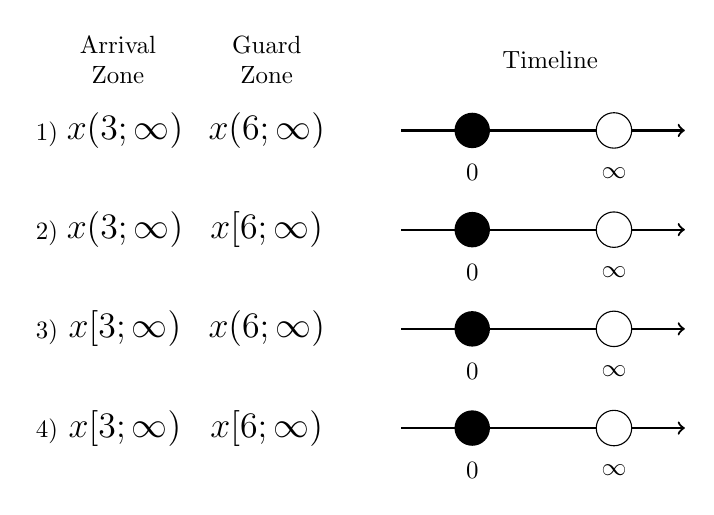
\begin{tikzpicture}[scale=0.9, every node/.style={scale=0.9}]

    \node[align=center] at (1,1) {Arrival \\ Zone};
    \node[align=center] at (3.1,1) {Guard \\ Zone};
    \node[align=center] at (7.1,1) {Timeline};
    \node at (0,-0.05) {1)};
    \node[font=\Large] at (1.1,0) {$\bm{x(3;\infty )}$};
    \node[font=\Large] at (3.1,0) {$\bm{x(6;\infty )}$};
    
    \node at (0,-1.45) {2)};
    \node[font=\Large] at (1.1,-1.4) {$\bm{x(3;\infty )}$};
    \node[font=\Large] at (3.1,-1.4) {$\bm{x[6;\infty )}$};
    
    \node at (0,-2.85) {3)};
    \node[font=\Large] at (1.1,-2.8) {$\bm{x[3;\infty )}$};
    \node[font=\Large] at (3.1,-2.8) {$\bm{x(6;\infty )}$};
    
    \node at (0,-4.25) {4)};
    \node[font=\Large] at (1.1,-4.2) {$\bm{x[3;\infty )}$};
    \node[font=\Large] at (3.1,-4.2) {$\bm{x[6;\infty )}$};
    
    
    \draw [thick ,->] (5,0) -- (9,0);
    \fill (6,0) circle (0.25);
    \draw[fill=white] (8,0) circle (0.25);
    \node at (6,-0.6) {$\bm{0}$};
    \node at (8,-0.6) {$\bm{\infty}$};
    
    \draw [thick ,->] (5,-1.4) -- (9,-1.4);
    \fill (6,-1.4) circle (0.25);
    \draw[fill=white] (8,-1.4) circle (0.25);
    \node at (6,-2) {$\bm{0}$};
    \node at (8,-2) {$\bm{\infty}$};
    
    \draw [thick ,->] (5,-2.8) -- (9,-2.8);
    \fill (6,-2.8) circle (0.25);
    \draw[fill=white] (8,-2.8) circle (0.25);
    \node at (6,-3.4) {$\bm{0}$};
    \node at (8,-3.4) {$\bm{\infty}$};
    
    \draw [thick ,->] (5,-4.2) -- (9,-4.2);
    \fill (6,-4.2) circle (0.25);
    \draw[fill=white] (8,-4.2) circle (0.25);
    \node at (6,-4.8) {$\bm{0}$};
    \node at (8,-4.8) {$\bm{\infty}$};
    \end{tikzpicture}

\caption{Four identical timelines for varying strictness of arrival and guard zones} \label{fig:tl-3}
\end{figure}

To fix these issues it would perhaps suffice to to enrich the timeline to be able to preserve more information that will be necessary in the phase of zone adjustment, however a new, more powerful concept was discovered.

\section{Global Zones}\label{sec:globalZone}
So far we have discussed a number of concepts such as arrival zone, Min/Max, accumulative delays and timeline, all of which shared similar problems - loss of information, impossibility of subtraction of opposite bound constraints and more. All of these previous concepts required a number of changes to perform correctly, however then they would become too unintuitive and cumbersome to implement.

This section presents the final concept that is used in the implementation of \jecdar - the one of the \textit{global zone}. As described in Section \ref{sec:refRules}, the refinement relation rules are applied on the pairs of the states that belong to the refinement relation. Each state in the state pair represents a number of corresponding locations and contains its own zone that keeps track of all clocks from relevant automata. It means that both left and right sides of the refinement (left and right states in the state pair) existed independently from each other. Having their own zones that could not be related or compared due to their potentially differing size, proper state-space exploration required some mechanisms for zone comparisons, all of which were described in previous sections.

Moreover, clocks of different sides of the refinement cannot be semantically compared. However, as was discovered later, such a mindset caught us locked in the tunnel vision trap.

\subsection{One common zone}
In fact, throughout the entire development of all the previous concepts, it appears that we were unconsciously trying to find various mechanism allowing us to compare every clock of the left side of the refinement to every clock on the right side. The "flattening" approach of the timeline was perhaps the closest concept to achieving that. Finally, the concept of a \textit{global} zone was born, which implies storing all clocks of the entire refinement in a single zone and thus having a single zone per refinement relation instead of two as before. 

The global zone helps to easily and efficiently solve a number of problems and allows us to freely use such DBM Library operations as \textsc{isSubsetEq}, \textsc{DbmMinusDbm} and \textsc{FedMinusFed} due to the global zone being of the same dimension (size) throughout the entire refinement. Moreover, storing all the clocks in one zone also implies constantly maintaining the relationship between any pair of clocks.

\subsection{Refinement rules verification}
With the global zone, the verification of refinement rules becomes a much more intuitive task. Consider the example in Figure \ref{fig:tl-refoutfail} where two automata are challenged to satisfy the refinement relation. The global zone, storing information about clocks of both sides of the refinement is used to verify refinement rules. For simplicity, axes \textbf{x} and \textbf{y} correspond to clocks \textbf{x} and \textbf{y} respectively. 

We know that the refinement output rule challenges an automaton on the right side of the relation to follow the left side with the same common output (in this example \textbf{o!}). To verify that, the global zone of the initial location is constrained by the corresponding guard ($x \leq 4)$ to obtain the zone of all the clock valuations when the output edge can be taken from \textbf{id0} to \textbf{id1} (zone on the left side). At this point, it is allowed to "cut" (constrain) the zone. Next, the resulting zone is then being constrained by the guard of the right side ($y \leq 2$). As can be seen on the right diagram of the zone (Figure \ref{fig:tl-refoutfail}), the application of the guard would not only constrain the clock of the right side \textbf{y}, but would also "cut" solutions from the clock of the left side \textbf{x}. This indicates that not for all the clock valuations an output can be taken on the left side so that the right side could follow. Therefore, refinement fails.

\begin{figure}
\centering
\begin{tikzpicture}[scale=0.9, every node/.style={scale=0.9}]
    %Automata
    \node at (1.6, 5.5) {\includegraphics{figures/gz-aut1.png}};
    \node at (9.4, 5.5) {\includegraphics{figures/gz-aut2.png}};
    \node[font=\Large] at (5.5,5.5) {$\Scale[2]{{\leq}}$};

    % Axis
    \draw [thick ,->] (-0.5,0) -- (3.5,0);
    \draw [thick ,->] (0,-0.5) -- (0,3.5);
    \node at (3.5,-0.4) {$\bm{x}$};
    \node at (-0.4,3.5) {$\bm{y}$};
    
    % X coordinates
    \draw [thick] (1.4,-0.1) -- (1.4,0.1);
    \node at (1.4,-0.4) {$\bm{2}$};
    \draw [thick] (2.8,-0.1) -- (2.8,0.1);
    \node at (2.8,-0.4) {$\bm{4}$};
    
    % Y coordinates
    \draw [thick] (-0.1,1.4) -- (0.1,1.4);
    \node at (-0.4,1.4) {$\bm{2}$};
    \draw [thick] (-0.1,2.8) -- (0.1,2.8);
    \node at (-0.4,2.8) {$\bm{4}$};
    
    % Diagional Lines
    \draw [thick] (0,0) -- (2.8, 2.8);
    \draw [thick, dotted] (2.8, 2.8) -- (3.2, 3.2);
    \node[green] at (3.5,1.4) {$\bm{x \leq 4}$};
    
    % Dotted lines
    \draw [thick, green, dashed] (2.8,0) -- (2.8, 3.5);
    
    
    \node at (5.5, 1.4) {$\Longrightarrow$};
    
    %Second Plot
    % Axis
    \draw [thick ,->] (7.5,0) -- (11.5,0);
    \draw [thick ,->] (8,-0.5) -- (8,3.5);
    \draw [thick, red] (9.4,0) -- (10.8,0);
    \node at (11.5,-0.4) {$\bm{x}$};
    \node at (7.6,3.5) {$\bm{y}$};
    
    % X coordinates
    \draw [thick] (9.4,-0.1) -- (9.4,0.1);
    \node at (9.4,-0.4) {$\bm{2}$};
    \draw [thick] (10.8,-0.1) -- (10.8,0.1);
    \node at (10.8,-0.4) {$\bm{4}$};
    
    % Y coordinates
    \draw [thick] (7.9,1.4) -- (8.1,1.4);
    \node at (7.6,1.4) {$\bm{2}$};
    \draw [thick] (7.9,2.8) -- (8.1,2.8);
    \node at (7.6,2.8) {$\bm{4}$};
    
    % Diagonal Lines
    \draw [thick] (8,0) -- (9.4, 1.4);
    \draw [thick, red, dotted] (9.4, 1.4) -- (10.8, 2.8);
    \node[red] at (10.5,1.1) {$\bm{y \leq 2}$};
    
    % Dotted lines
    \draw [thick, red, dashed] (8,1.4) -- (11.5, 1.4);
    
\end{tikzpicture}
\caption{Refinement fails due to its output rule being not satisfied. Global zones illustrated after application of guards. Zone of the right side "cuts" solutions from the left side.} \label{fig:tl-refoutfail}
\end{figure}

Algorithmically, the easiest way to discover that a zone was "cut" is to make use of the subtraction operation \textsc{DbmMinusDbm} provided by the DBM Library. If the result of such a method call results in anything but an empty zone, it indicates that solutions were lost. Thus, the verification of the refinement output rule requires the subtraction of the right side global zone from the left side one, whereas the refinement input rule requires the opposite.

Moreover, the concept of the global zone removes any necessity to keep track of accumulative delays, which were described in Section \ref{sec:accumDelays}. This is due to the fact that zones contain not only lower and upper bounds of the clock, but also the relationship between any pair of clocks. In such cases as in Figure \ref{fig:accDelay}, if constructed properly the global zone would maintain the difference between clocks and the accumulative delays can then also be verified with the help of zone subtraction. A similar logic applies to the verification of the refinement delay rule, with a difference in subtraction being used on the global zones after the application of the corresponding invariants.

\subsection{Extrapolation}
During the verification of the refinement, the \textit{passed} list of states is used to guarantee termination. Whenever a new state is explored, it is checked against the existing \textit{passed} list with the following conditions: the locations of the compared states should be equal and the zone of the new state should be a subset of the state in the \textit{passed} list. If both of these conditions hold, the newly discovered state is considered as "already explored" and is discarded. This approach used to guarantee termination when each side of the refinement had its own zone.

However, the introduction of the global zones came along with another challenge. In some cases, the state-space exploration algorithms would no longer terminate due to the zone being infinitely incremented. Figure \ref{fig:gz-extrapolation} shows a simple example of this. Notice the invariant ($x \leq 1$) and the reset ($x=0$) that is present on the left side of the refinement, but not on the right. During state-space exploration we would expect the algorithm to terminate as in principle no new zones or locations are discovered even after the first traversal of \textbf{o!} edge on any side. However this is not the case for the global zones.

\begin{figure}
\centering
\begin{tikzpicture}[scale=0.9, every node/.style={scale=0.9}]
    %Automata
    \node at (0, 0) {\includegraphics{figures/gz-extr-a1.png}};
    \node at (5, 0.25) {\includegraphics{figures/gz-extr-a2.png}};
    \node[font=\Large] at (2.5,0) {$\Scale[2]{{\leq}}$};
    
\end{tikzpicture}
\caption{Refinement example that requires extrapolation techniques to terminate.} \label{fig:gz-extrapolation}
\end{figure}

Since global zones also preserve information about relationship between clocks during the state-space exploration, the zone would keep progressively moving upwards on the \textbf{y} axis. Thus, the termination of the algorithm would not be possible due to an infinite number of symbolic states. 

To cope with this problem in \jecdar, a zone-based abstraction technique, also known as \textit{extrapolation}, (\textcite{ExtrapolationLU}) is used. Apart from \uppaal, extrapolation is also used in such tools as \textsc{Kronos} and \textsc{RtSpin} where it is referred to as \textit{maximization} (\textcite{maximization}). While preserving reachability properties, extrapolation greatly reduces the state-space that needs to be explored.

Extrapolation is based on the idea that the outcome of the feature verification for automata is only affected by the changes to a clock if its value is below some certain constant. As soon as the clock has surpassed the constant its values become irrelevant, i. e. all further resulting states are identical except for clock valuations exceeding the maximum constant. 

The selection of the maximal constants for clocks is an important matter as it influences the coarseness of the abstraction - the smaller the constant, the smaller state-space that has to be explored and less time and memory has to be used for the  verification of properties. 
The choice of the constant $k$ involves static analysis of the automaton with the aim of finding the maximal constant appearing in either guards or invariants within the structure of the automaton. Currently \jecdar finds one such constant for each of the clocks, which is a much coarser abstraction that using a single constant. In the example of Figure \ref{fig:gz-extrapolation} the maximal such constant for clock \textbf{x} is $k = 1$. As soon as the upper bound of that clock in the zone is greater than $k$ it is considered insignificant and can be replaced by a higher value being either the next highest upper bound of any another clock in the zone or an infinity if none. 

The idea of extrapolation has also been taken further in a number of studies to construct coarser yet exact abstractions. For example in \textcite{StaticGuardAnalysis} in addition to a constant depending on a particular clock it also depends on a particular location of the automaton. However, the current implementation of \jecdar makes use of the extrapolation based on the maximal constants for clocks, which is a potential subject for improvement in the future work.